%************************************************
\chapter{Design}\label{ch:design} % $\mathbb{ZNR}$
%************************************************
As stated in the introduction (\autoref{ch:introduction}), the research question is the following: ``How can the cost and waste monitoring of a Cloud Computing application be offered in a scalable and resilient manner?''. In order to investigate the characteristics of the solution for monitoring a Cloud Computing application, it is important to determine the requirements before. The requirements are divided into architectural requirements and waste requirements. The architectural requirements will lead to the proposed architecture, while the waste requirements will lead to a specified algorithm.

\section{Architectural requirements} \label{sec:architectural_req}
As this research is the successor of the work: `Visualizing Computational Waste in Cloud Computing' by A. Spina \cite{spina}, there is some similarity with his architectural requirements. However, his architecture is based on a solution for which a probe collects data from monitored instances, and an aggregator that represents this data into a human-readable format. His relevant requirements are:
\begin{itemize}
    \item The solution should be functional across command cloud providers.
    \item The data should be considered sensitive and secured accordingly.
    \item The solutions should be configurable, but easy to use.
    \item The solution should strike a balance between efficiency and effectiveness.
    \item The solution should collect utilization statistics on the monitored system. 
\end{itemize}

\noindent
In \cite{aceto2013cloud} a number of properties are mentioned. These apply to a distributed monitoring system, and are therefore applicable to the desired solution. The most important properties are:
\begin{itemize}
    \item Scalability: a monitoring system is scalable if it can cope with a large number of probes.
    \item Elasticity: a monitoring system is elastic if it can cope with dynamic changes of monitored entities, so that virtual resources created and destroyed by expansion and contraction are monitored correctly.
    \item Adaptability: a monitoring system is adaptable if it can adapt to varying computational and network loads in order not to be invasive.
    \item Timeliness: a monitoring solution is timely if detected events are available on time for their intended use.
    \item Autonomicity: an autonomic monitoring solution is able to self-manage its distributed resources by automatically reacting to unpredictable changes.
    \item Accuracy: a monitoring system is accurate when the measures it provides are accurate, i.e. they are as close as possible to the real value to be measured.
\end{itemize}

\noindent
Both lists in this section are considered relevant, and the desired solution should be able to meet all these properties. For the implemented solution, the decision has been made to monitor only Docker containers, as this provides a way of abstracting a certain deployment. Therefore, the underlying operating system is not that important. This ensures that the solution will be functional across all OS's that are capable of running Docker containers. 

\section{Architecture} \label{sec:architecture}
As mentioned in \autoref{sec:related_technologies}, the proposed architecture uses state-of-the-art open-source technologies. Several design patterns have been evaluated, such as a Client-Server network and a peer-to-peer network. the latter is considered more scalable, as the number of resources grow with the number of nodes. Additionally, a peer-to-peer system does not have a single point of failure. Therefore, this system is desired over a client-server network. However, as the data is stored in a Prometheus database, and this cannot operate in a peer-to-peer system, another solution is needed. Using the federation technique of Prometheus \cite{prometheus_federation}, the decision has been made to go for a hierarchical network. This proposed network consists of only one root, a number of supernodes, and optional a number of nodes.\\

\noindent
An architectural overview of the three node types, as well as the technologies that are included, can be found in \autoref{fig:architecture}. Several processes are listed in bold as this denotes a custom created process. The only difference between a node and a super node is the Prometheus database. Furthermore, the root is only used to visualize the collected metric data in the Grafana dashboard. Each node type is shortly described below.

\begin{figure}
    \centering
    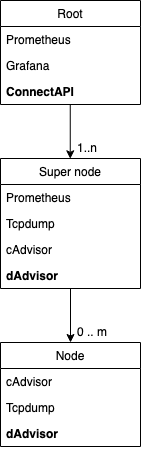
\includegraphics[width=0.3\textwidth]{gfx/architecture.png}
    \caption{Architectural overview}
    \label{fig:architecture}
\end{figure}

\subsection{Root}
The root is a single access point for the displaying the obtained results. Its Prometheus database is dynamically configured, such that it scrapes data from all the super nodes deployed in the system. 
In order to successfully deploy the entire system, the root needs to be deployed first, as it provides an access point for the nodes as well. This access point is implemented in the connect API and further described in ....\todo{add reference}. The connect API distributes the available nodes over the available super nodes and ensures that $\floor*{\frac{n}{m}} \leq \frac{n}{m} \leq \ceil*{\frac{n}{m}}$ holds for which $n$ is the number of nodes and $m$ the number of super nodes.

\subsection{Super node}
As explained before, there is only a slight difference between a node and a super node, as the latter deploys Prometheus. This database is automatically configured such that is scrapes from a set of nodes (as received from the root). The metrics that a super node collects are the same as for a node and are therefore described in the following section.

\subsection{Node}
The node consists of three processes. Resource metrics (i.e. CPU and memory) are collected using the cAdvisor process and internet packets are collected using Tcpdump \cite{tcpdump}. This data is collected using the dAdvisor process, which acts as an aggregator. This process ensures that the data is correctly formatted, and makes it available for Prometheus.


\section{Waste requirements} \label{sec:waste_requirements}
The CPU and memory are resource metrics that can be specified per Docker container. For a specific node, the sum of these metrics over all containers on that node is denoted as the total utilization. For these totals, there are a few restrictions, which are mathematically stated below.

\begin{itemize}
    \item $0 < u_i \leq 1$ for $1 \leq i \leq n$: Every container on a node utilizes a value between 0 (exclusive) and 1 (inclusive). The desired solution will also be a running container, but the utilization is filtered out of the collected utilization values, such that the monitoring solution only collects data about the deployed system.
    \item $\sum_{i=1}^n u_i \leq 1$: The total utilization of a certain set of containers for a given host cannot utilize more than 100\%. And with the previous requirement, its lower-bound is 0 (exclusive). As the total waste is computed as $1 - \sum_{i=1}^n u_i$, it can be concluded that the waste is bounded by 0 (inclusive) and 1 (exclusive).
\end{itemize}

\noindent
Although the mathematical constraints are very trivial, it is important to state this beforehand. Using these utilization requirements, several approaches of computing the resource waste can be assessed. Also, stating these constraints are important as it affects the desired solution.\\

There are several ways in which the utilization values can be used to compute the waste. In this research, the following three properties are used for finding an optimal waste distribution:
\begin{enumerate}
    \item \textbf{$\sum_{i=1}^n w_i = 1 - \sum_{i=1}^n u_i $}: The sum of the elements of the waste and the sum of the elements of the utilization values should sum up to 1, as it implies that a resource is either used (this is $u$) or being wasted (this is $w$).
    \item \textbf{$w_i \geq 0$} for $1 \leq i \leq n$: The waste of every certain container is non negative. Thus, it is impossible for a container to have a negative waste. As the waste distribution is used for computing the amount of money to be wasted, this would imply that money is being earned, while running a certain container.
    \item \textbf{$\max w_i \Rightarrow \min u_i$}: The container that utilizes the most resources, should be responsible for wasting the least amount of resources. This property implies that the order of containers from lowest utilization to highest utilization is the same as the order of containers from highest waste to lowest waste. 
    \item \textbf{$w_i = w_j \iff u_i = u_j$}: If two containers utilizes the same amount of resources, than they should also waste the same amount of resources. The opposite should also hold. If two containers utilizes both a different amount of resources, than it should also have a different amount of waste.
\end{enumerate}

The following section contains several different approaches for computing the waste distribution. In the section that follows this, the approaches are evaluated against the properties above.

\section{Approaches for computing the waste distribution} \label{sec:approaches}
In this section, the following three waste distributions will be evaluated: equal distribution, linear inverse distribution and proportional inverse distribution. They are all described in a different subsection below.

\subsection{Equal distribution} \label{sec:equal}
Using an equal distribution, the waste is the same for every container on a certain host, i.e. $w_1 = w_2 = \dots = w_n$. The idea behind this approach is that a set of containers together wastes the same part of the host and therefore the waste should be distributed over every container in a fair manner. This approach can be computed by the following formula:
\begin{equation}
w_i = \frac{1 - \sum_{i=1}^n u_i}{n}
\end{equation}

\subsection{Linear inverse distribution} \label{sec:linear}
This distribution computes a higher waste for a container that utilizes less, and can be computed by the following formula:
\begin{equation} \label{eq:linear}
w_i = \frac{1}{n} - u_i
\end{equation}
However, it is easy to see that \autoref{eq:linear} returns a negative value if $u_i > \frac{1}{n}$ (contradicts property 2). Therefore, this formula can be replaced by the following formula:
\begin{equation}\label{eq:heuristic}
w_i = \begin{cases}
\frac{1}{n} - u_i & \text{if } u_i \leq \frac{1}{n}\\
0                 & \text{otherwise}
\end{cases}
\end{equation}
This yields another problem, as it is not guaranteed that property 1 holds. In fact, property 1 will fail, if there exists a $j$ for which $u_j > \frac{1}{n}$ (the function returns the \textit{otherwise}-case). Therefore, a simple formula can be used to restore property 1. Note that $u = \sum_{i=1}^n u_i$ and $w = \sum_{i=1}^n w_i$ and needs to be computed before the first $w_i$ is updated.
\begin{equation} \label{eq:update}
w_i \leftarrow w_i * \frac{1-u}{w}
\end{equation}
An example for $n = 2$ can be the following distribution $u_1 = 0.6$ and $u_2 = 0.3$. After \autoref{eq:heuristic}, the following values are found $w_1 = 0$ and $w_2 = 0.2$. However, since property 1 doesn't hold, $w_2$ is updated to $0.1$. The entire algorithm for this approach is formulated in Algorithm \ref{alg:linear}.

\begin{algorithm}
    \caption{Compute the waste based on the linear inverse distribution}\label{alg:linear}
    \begin{algorithmic}[1]
        \Procedure{computeWaste}{$u_1, u_2, \dots, u_n$}
        \For{$i \gets 1 \dots n$}
        \State $w_i\gets \max(\frac{1}{n} - u_i,~0)$
        \EndFor
        \State $u\gets \sum_{i=1}^n u_i$
        \State $w\gets \sum_{i=1}^n w_i$
        \If{$u+w \neq 1}$
        \For{$i \gets 1 \dots n$}
        \State $w_i\gets w_i * \frac{1-u}{w}$
        \EndFor
        \EndIf
        \State \textbf{return} $w_1, w_2, ..., w_n$
        \EndProcedure
    \end{algorithmic}
\end{algorithm}


\subsection{Proportional inverse distribution} \label{sec:proportional}
This distribution uses the idea that the product of the utilization and the waste distribution should be constant for every container. 
The formula is therefore: $w_i * u_i = c$ for an unknown value of $c$. This implies that if a certain container utilizes a high amount of resources, its corresponding waste must be a low number.
The $c$-value is constant across all containers on a specific host, which leads to the general formula: 
\begin{equation} \label{eq:constant}
w_1 * u_1 = w_2 * u_2 = \dots = w_n * u_n
\end{equation}
However, in case of $n = 1$, there is no equation possible. In this case, the waste can directly be computed using property 1, and thus $w_1 = w = 1 - u_1$.

In general (for $n \geq 2$), \autoref{eq:constant} results in $n-1$ unique equations. However, this set of equations cannot be solved, as there are $n$ variables unknown ($w_1$ to $w_n$). But property 1 can be used to generate $n$ unique equations. For example, for $n=3$ the following equations needs to be solved:
\begin{equation}\label{eq:linear3}
\begin{split}
w_1 & u_1 - w_2 * u_2 &= 0 \\
w_1 & u_1 - w_3 * u_3 &= 0 \\
w_1 + w_2 + w_3 &= 1 - u_1 - u_2 - u_3
\end{split}
\end{equation}
This system of linear equations can be represented by a matrix equation of the form $Ax = b$:
\begin{equation} \label{eq:matrix}
\begin{split}
A x &= b\\
\begin{bmatrix}
u_1 & -u_2 & 0    \\
u_1 & 0    & -u_3 \\
1   & 1    & 1
\end{bmatrix}
\begin{bmatrix}
w_1 \\ w_2 \\ w_3
\end{bmatrix}
&= \begin{bmatrix}0 \\ 0 \\ 1 - \sum_{i=1}^3 u_i\end{bmatrix}
\end{split}
\end{equation}

\autoref{eq:matrix} can be generalized for $n$ containers. The matrix $A_n$, as well as vectors $w$ (was $x$ in \autoref{eq:matrix}) and $b$ are expressed below:
\begin{equation} \label{eq:general_matrix}
\begin{split}
A_n &= \begin{bmatrix}
u_1    & -u_2 &       &        & \\
u_1    &      &  -u_3 &        & \\
\vdots &      &       & \ddots & \\
u_1    &      &       &        & -u_n \\
1      & 1    & 1     & \dots  & 1 \\
\end{bmatrix}
\end{split}
\begin{split}
w &= \begin{bmatrix}w_1 \\ w_2 \\ \vdots \\ w_{n-1} \\ w_n\end{bmatrix}
\end{split}  
\begin{split}
b = \begin{bmatrix}
0 \\ 0 \\ \vdots \\ 0 \\ 1 - \sum_{i=1}^n u_i
\end{bmatrix}
\end{split}
\end{equation}

Thus, the waste values can be computed by solving $A_n w = b$. 
In general, the following two properties needs to hold to have a unique solution given by $w = A_n^{-1} b$:
\begin{itemize}
    \item \textbf{The matrix is a square}: this holds, as $A_n$ has $n$ rows and $n$ columns.
    \item \textbf{The matrix has full rank (all rows are linearly independent)}: this also holds, as this is how matrix $A_n$ was constructed from the equation in \autoref{eq:linear3}.
\end{itemize}
Therefore, the matrix $A$ is invertible. This also implies that its determinant is non-zero. This also holds and is proven in \autoref{ch:proof}. Thus, $A^{-1}$ can always be constructed, and this implies that $w$ can always be solved.

 